\documentclass{article}
\usepackage[utf8]{inputenc}
\usepackage[english]{babel}
\usepackage{graphicx}
\title{Lab Report for HippyLearn-s CNN Model}
\author{Haocheng An}
\date{February 24 2018}

\begin{document}
	
	\maketitle
	\section{Introduction}
	We are faced with hippylearn-s model to use Deep CNN to solve the helmholtz problem. 
	\section{Methodology}
	I tried 3 different types of neural networks, that is monotonically increasing in number of channels, monotonically decreasing and the increasing first and then decrease. We get the number as specified below. For each kind of neural network, I also try 2 different kinds of activation functions: relu $$f(x) = x >0 ? x: 0$$ the softplus$$f(x) = ln(1+ e^{x})$$
	For the fairness, we take the batch size and the nfeatures to be 888 and 32 resectively.
	\section{Result}
	\par 
	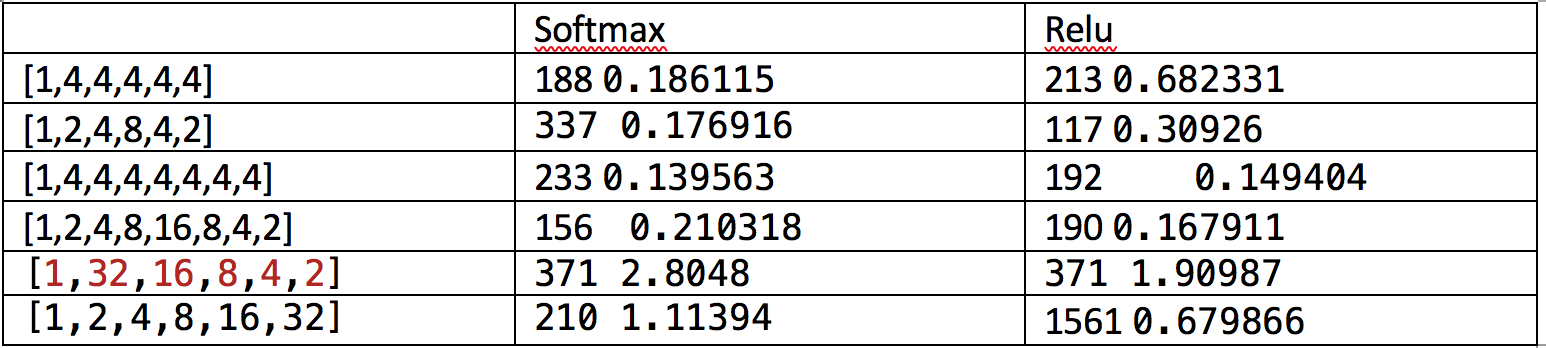
\includegraphics[width=135mm,height=50mm]{general.png}
	The result above indicates that for bigger neural networks, the relu works better than softplus as actiavation function.
	The first integer in this column reflects the number of iterations needed to converge such that the difference between two adjacent iteration is smaller than $10^{-4}$
	Also, when comparing the neural networks of using same activation functions, the monotonic decreasing or increasing model not work as good as the non-monotonic one. In other words, the first increasing then decreasing model offer us lower training loss. With the thought given above, we compare more models of similar increasing and decreasing with different activation functions and see how it behaves. (To be continued with this part, still training)
	\par I also tried different activation functions and different optimizer for a given structure of the neural nets.
	tf.nn.relu 0.08
	tf.nn.softmax 0.1759
	tf.nn.elu 0.9733
	tf.nn.elu gradient descent 0.07
	
	\section{Future Work}
	\par With the comparison made above, activation functions and structure of the network can have some effects on the accuracy and training efficiency. For the future, we can also change the optimizer functions, for example, integrate the momentum optimizer inside and it may probide better result.
\end{document}